% ----------------------------------------------------------------------
%  Pracovní úkoly
% ----------------------------------------------------------------------
\section{Pracovní úkoly}

\begin{enumerate}
\item Pro tři vodorovné trubice s různými poloměry kruhového průřezu, které jsou opatřeny manometry, změřte závislost objemového průtoku Qv na úbytku statického tlaku \(\Delta p\) na vyšetřované délce trubice l ve směru proudění.

\item Sestrojte graf závislosti \(Qv = Qv(p).\)

\item Ze směrnice závislosti \(Qv = Qv(p)\) v oblasti laminárního proudění určete poloměr trubice.

\item Upravený poloměr dosaďte do vztahů pro výpočet Re a k.

\item Sestrojte graf závislosti k = k(Re), kde k je součinitel odporu trubice a Re je Reynoldsovo číslo. Do grafu vyneste teoretickou závislost pro laminární i turbulentní proudění.
\end{enumerate}

% ----------------------------------------------------------------------
%  Teoretická část
% ----------------------------------------------------------------------
\section{Teoretická část}

    Pro studium závislosti objemového průtoku \(Q_V\) na úbytku statického tlaku \(\Delta p\) použijeme aparaturu znázorněnou na obr. \ref{fig:schema}. Díky této závislosti určíme i oblasti laminárního a turbulentního proudění. Změnou rychlosti proudění vody v trubici se mění výška hladiny v manometru. Úbytek statického tlaku je dán vztahem

    \begin{equation}
        \Delta p = h\rho g,
    \end{equation}

    kde \(\rho\) je hustota kapaliny a \(g\) je místní tíhové zrychlení.

    \begin{figure}[h]
        \centering
        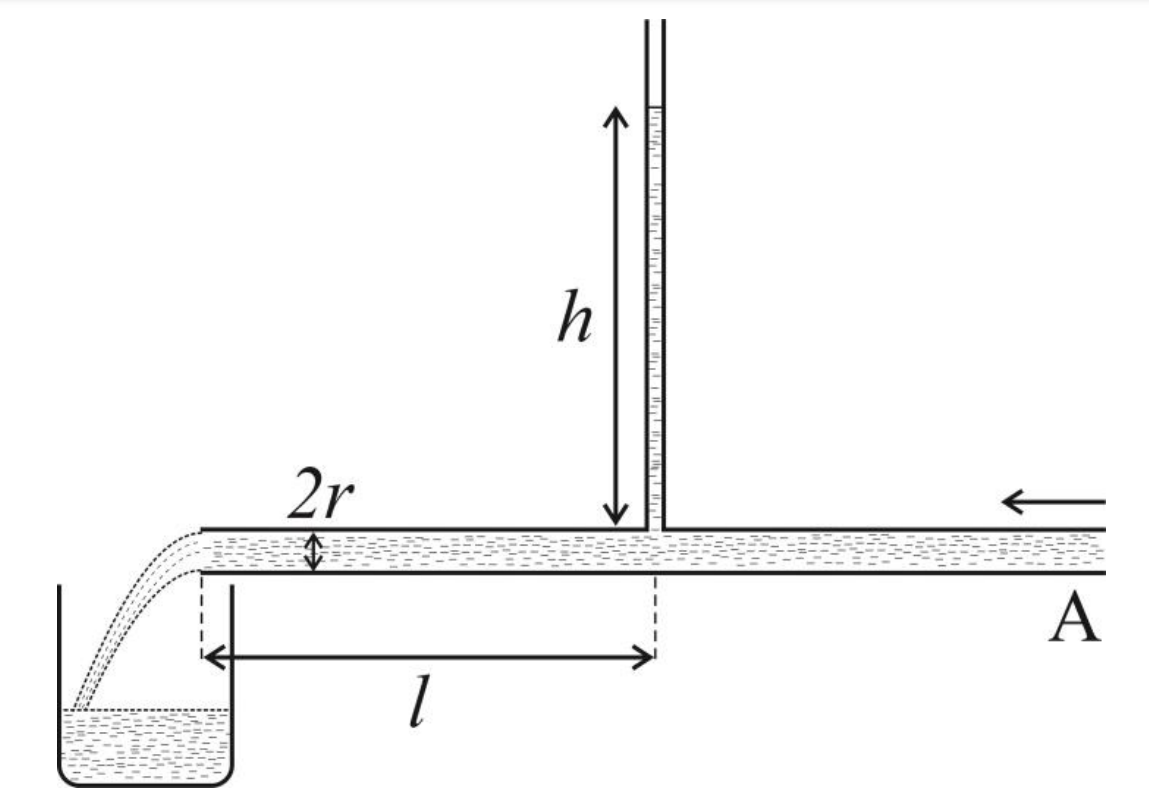
\includegraphics[width=0.5\linewidth]{01 - Studium proudění viskózní kapaliny trubicemi kruhového průřezu//Protokol//img/Schéma.png}
        \caption{Schéma zařízení.}
        \label{fig:schema}
    \end{figure}

    Objemový průtok je dán vztahem

    \begin{equation}
        Q_V = \frac{V}{t},
    \end{equation}

    kde \(V\) je objem kapaliny proteklé trubicí za čas \(t\).

    V oblasti laminárního proudění pro objemový průtok platí Poiseuillova rovnice

    \begin{equation}
        Q_V = \frac{\pi r^4}{8\eta l}\Delta p,
    \end{equation}

    kde \(r\) je vnitřní poloměr, \(l\) délka trubice a \(\eta\) dynamická viskozita proudící kapaliny.

    Proudění je laminární pokud nepřekročí kritickou hodnotu Reynoldsova čísla

    \begin{equation}
        Re = \frac{r\rho v_s}{\eta},
    \end{equation}

    kde \(v_s\) je střední rychlost proudění v trubici.

    Pro laminární proudění platí teoretický vztah

    \begin{equation}
        k = \frac{16}{Re},
    \end{equation}

    kde k je součinitel odporu trubice.
% ----------------------------------------------------------------------
%  Výsledky a zpracování měření
% ----------------------------------------------------------------------
\section{Výsledky a zpracování měření}

% ----------------------------------------------------------------------
%  Diskuse výsledků
% ----------------------------------------------------------------------			
\section{Diskuse výsledků}

% ----------------------------------------------------------------------
%  Závěr
% ----------------------------------------------------------------------
\section{Závěr}
